\documentclass[12pt]{article}\usepackage[]{graphicx}\usepackage[]{color}
%% maxwidth is the original width if it is less than linewidth
%% otherwise use linewidth (to make sure the graphics do not exceed the margin)
\makeatletter
\def\maxwidth{ %
  \ifdim\Gin@nat@width>\linewidth
    \linewidth
  \else
    \Gin@nat@width
  \fi
}
\makeatother

\definecolor{fgcolor}{rgb}{0.345, 0.345, 0.345}
\newcommand{\hlnum}[1]{\textcolor[rgb]{0.686,0.059,0.569}{#1}}%
\newcommand{\hlstr}[1]{\textcolor[rgb]{0.192,0.494,0.8}{#1}}%
\newcommand{\hlcom}[1]{\textcolor[rgb]{0.678,0.584,0.686}{\textit{#1}}}%
\newcommand{\hlopt}[1]{\textcolor[rgb]{0,0,0}{#1}}%
\newcommand{\hlstd}[1]{\textcolor[rgb]{0.345,0.345,0.345}{#1}}%
\newcommand{\hlkwa}[1]{\textcolor[rgb]{0.161,0.373,0.58}{\textbf{#1}}}%
\newcommand{\hlkwb}[1]{\textcolor[rgb]{0.69,0.353,0.396}{#1}}%
\newcommand{\hlkwc}[1]{\textcolor[rgb]{0.333,0.667,0.333}{#1}}%
\newcommand{\hlkwd}[1]{\textcolor[rgb]{0.737,0.353,0.396}{\textbf{#1}}}%

\usepackage{framed}
\makeatletter
\newenvironment{kframe}{%
 \def\at@end@of@kframe{}%
 \ifinner\ifhmode%
  \def\at@end@of@kframe{\end{minipage}}%
  \begin{minipage}{\columnwidth}%
 \fi\fi%
 \def\FrameCommand##1{\hskip\@totalleftmargin \hskip-\fboxsep
 \colorbox{shadecolor}{##1}\hskip-\fboxsep
     % There is no \\@totalrightmargin, so:
     \hskip-\linewidth \hskip-\@totalleftmargin \hskip\columnwidth}%
 \MakeFramed {\advance\hsize-\width
   \@totalleftmargin\z@ \linewidth\hsize
   \@setminipage}}%
 {\par\unskip\endMakeFramed%
 \at@end@of@kframe}
\makeatother

\definecolor{shadecolor}{rgb}{.97, .97, .97}
\definecolor{messagecolor}{rgb}{0, 0, 0}
\definecolor{warningcolor}{rgb}{1, 0, 1}
\definecolor{errorcolor}{rgb}{1, 0, 0}
\newenvironment{knitrout}{}{} % an empty environment to be redefined in TeX

\usepackage{alltt}
\usepackage{todonotes}
\usepackage[margin=1.2in]{geometry}
\usepackage{amssymb,amsmath,amsthm,graphicx}
\usepackage{enumerate}

\newtheorem{assump}{Assumption}[section]
\newtheorem{pro}{Proposition}[section]
\newtheorem{lem}{Lemma}[section]
\newtheorem{thm}{Theorem}[section]
\newtheorem{cor}{Corollary}[section]
\newtheorem{ineq}{Inequality}[section]
\newtheorem{defn}{Definition}[section]
\newtheorem{rem}{Remark}[section]
\newtheorem{ex}{Example}[section]
\theoremstyle{definition}
\newtheorem{alg}{Algorithm}[section]

\linespread{1.2}

\title{JMP Revisions Following Econometrica Comments}
\author{Francis J.\ DiTraglia}
\IfFileExists{upquote.sty}{\usepackage{upquote}}{}
\begin{document}

\maketitle

\begin{abstract}
This document collects all of the new material that I plan to add to my JMP following the referee reports from Econometrica. Once I've put this material together, I'll merge it with the existing version and send it to ReStud.
\end{abstract}

\section*{Referee Comments and My Responses}
The two main objections to my paper were as follows:
  \begin{enumerate}
    \item The FMSC provides an asymptotically unbiased estimate of MSE, but the FMSC itself is random, even in the limit. It is not true that the FMSC converges in probability to actual AMSE because of this additional randomness. 
    \item If the valid model is identified, why not just use it? If it's not identified, FMSC doesn't work. It's not clear that the gains from this procedure would be large in practice since the FMSC has a variance. See point \# 1. 
    \item This approach is not robust to weak identification.
    \item The procedure for correcting confidence intervals is too computationally intensive and aims to get the size correct without even looking at the width.
    \item Finite sample MSE doesn't always exist for these kinds of models. Maybe this isn't the best measure to look at.
    What about OLS versus IV?
    \item There are some missing references.
    \item Some objections to the simulation experiment. In particular, no widths are reported for confidence intervals.
  \end{enumerate}
The most important objections are 1 and 2, possibly followed by 3. The other points can be fairly easily dealt with and I will do so below. 

\paragraph{Objection \# 1} This comment boils down to ``I don't like efficient model selection: you should use consistent model selection.'' It is indeed true that the FMSC is random even in the limit and that it does not converge to actual AMSE: it is merely an asymptotically unbiased estimator of AMSE. However, this is the whole point: I explicitly want to \emph{avoid} doing consistent selection because the associated risk properties are so poor. I need to make this clearer by citing, for example, the Leeb and P\"{o}tscher paper from 2008 that Larry Wasserman discussed on his blog.

In a certain sense, this comment amounts to a critique of my use of local asymptotics. I should make very clear that this device is widely used in econometrics to study, among other things, local power, local-to-unit roots, etc. I should provide references for this, including Schorfheide and Moon. Furthermore, a great many model selection procedures are random in the limit: Mallows $C_p$ and AIC are two well-known examples, but many people have worked with selection in this framework. I should cite Bruce Hansen as well as Frank Schorfheide's VAR paper and Schorfheide and Moon.

I should also relate my framework to the idea of uniform asymptotic validity as discussed in Andrews and Guggenberger (2010) and Schorfheide and Moon.


\paragraph{Objection \# 2} This comment suggests that: (a) my simulations weren't convincing enough, and (b) I wasn't clear enough about the sort of situation for which the FMSC is designed. The solution is to do more and better simulations and to be clearer! The point of the FMSC is that we often find ourselves in a setting where there are various ``plausible'' assumptions we could use in estimation, some of which are weaker and some of which are stronger. Typically, we worry that the weaker assumptions might not provide sufficient information to study the question we're interested in, which we worry that the stronger assumptions might not quite be true. You can think of this as a kind of ``prior knowledge'' that violations of the stronger assumptions are ``small'' which is pretty much exactly what the local mis-specification idea encodes. I can relate this to the idea of ``plausibly exogenous'' as well as Schorfheide and Moon. 

I should be clear about the fact, and I need to find the citation for this, that model selection cannot uniformly beat the ``full'' model. (In this case, the full model is the set of moment conditions based on the weakest assumptions.) However, selection \emph{can} beat the ``full'' model over large regions of the parameter space, so it's really a questino of where you think you might be a priori. I should argue that the whole idea is to use my method when you consider it likely that you might be in the relevant region of the parameter space. I should also show in simulations that the cost you pay when you are \emph{not} in this region isn't too high.


\paragraph{Objection \# 3} This point is less important but also harder to handle. I'm pretty sure that there's no straightforward way to include weak identification in my framework directly although it's a very compelling idea: when you have weak identification it might make a lot of sense to use a slightly endogenous instrument. Even though I don't think it's possible to incorporate weak instrument \emph{asymptotics}, however, I can still evaluate how my proposed \emph{procedure} deals with weak instruments. There are at least two ways to do this. The first is by carrying out a simulation study. The second is by looking trying to relate the FMSC to some other well-known tests or procedures. In the IV versus OLS case, for example, I know that the result is a Hausman test with a non-standard critical value. I seem to recall that Dufour has a paper in which he argues that this is a good idea when you might have weak instruments. Basically the idea here is to look at how the FMSC implicitly trades off instrument strength and validity when we take the procedure \emph{outside} of its asymptotic framework.  

\paragraph{Overall Thoughts and To Do List}
Besides responding to the Objections 1--3, here are some other things I should do, roughly in order of importance:
  \begin{enumerate}
    \item Should defend my assumption that we have a minimal set of correct MCs by referencing the literature, including Chen etc.
    \item Change the notation to allow us to use arbitrary subsets of the moment conditions. This will accomodate the OLS/IV example.
    \item Allow the weighting matrix $W$ to be indexed by $S$.
    \item Fold in the IV/OLS example. This will allow me to discuss a number of interesting points, including optimal estimator averaging, weak instruments, relationship to testing, etc. Also allows a brief consideration of what happens when we have no valid moment conditions.
    \item Do a better job with the choosing instruments example.
    \item New and better simulation experiments. Look at median absolute deviation as well as trimmed MSE, etc. Try to cover more of the parameter space, etc. Pictures rather than tables. Everything needs to be replicable for ReStud!
    \item Re-do the empirical example with improved code for the confidence interval. Everything needs to be replicable for ReStud!
    \item Possibly add a second empirical example for OLS versus IV.
    \item Look at the proposed references and think about including them.
    \item Might want to be slightly more careful about regularity conditions. See for example Schorfheide and Moon.
  \end{enumerate}

\section{New Notation for Moment Selection Vector}
This is straightforward: just need to redefine $S$ and $\Xi_S$. See the GFIC paper.

\section{Two Running Examples in the Paper}
Two simple but empirically relevant examples we'll consider throughout the paper. Helpful because they make the intuition clear and also interesting in their own right. To be clear, FMSC applies to GMM in general, not just to linear models like these.


\paragraph{Example \#1: Choosing Instrumental Variables}
Consider the linear model
  \begin{equation}
  y_i = \mathbf{x}_i'\beta + \epsilon_i
  \end{equation}
where some or all of the regressors are endogenous. Suppose we have a vector of valid instruments $\mathbf{z}^{(1)}_i$ and another vector of ``suspect'' instruments $\mathbf{w}_i$ that are likely to be highly relevant but may well be slightly endogenous. These could be ``plausibly exogenous.'' Should we include $\mathbf{z}_i$ in the instrument set for use in estimation?  Arises in various settings. One concerns exogeneity assumptions in a panel data setting: strict exogeneity versus predeterminedness. 

\paragraph{Example \#2: Least Squares versus Instrumental Variables}
This example is similar to the first one, but illustrates that we don't have to structure the problem in terms of choosing over-identifying restrictions: we can select over fundamentally different estimators. Suppose we want to estimate the effect of an endogenous regressor $x$ in a linear model of the form
  \begin{equation}
    y_i = \mathbf{w}_i' \theta + \beta x_i + \epsilon_i
  \end{equation}
where $\mathbf{w}_i$ is a vector of endogenous control regressors. In this case the target parameter is $\beta$. Suppose we have a vector of valid instruments $\mathbf{z}_i$. Should we use OLS or IV? Dufour: ``IV is like Amputation; it should be a last resort to save the patient." Easily generalized to more than one endogenous regressor, but this example is very common in many settings, particularly treatment effects with microdata. Cite the Nevo and Rosen and Plausibly Exogenous papers. Another issue is weak instruments and whether it is possible to \emph{combine} OLS and IV.



\section{Local Mis-specification for the Examples}

\paragraph{Example \#1: Choosing Instrumental Variables}
 \begin{equation}
  E_n\left[\begin{array}{c}
    \mathbf{w}_i(y_i - \mathbf{x}_i \beta)\\
     \mathbf{z}_i(y_i - \mathbf{x}_i \beta)
  \end{array} \right] = \left[ \begin{array}{c}\mathbf{0} \\ \boldsymbol{\tau}/\sqrt{n} \end{array}\right] 
 \end{equation}
 
 \paragraph{Example \#2: Least Squares versus Instrumental Variables}
\begin{equation}
    E_n\left[\begin{array}{c}
    \mathbf{w}_i(y_i - \mathbf{w}_i' \theta  - \beta x_i)\\
    \mathbf{z}_i(y_i - \mathbf{w}_i' \theta  - \beta x_i)\\
    x_i(y_i - \mathbf{w}_i' \theta  - \beta x_i)
    \end{array}\right] = \left[\begin{array}{c} \mathbf{0} \\ \mathbf{0} \\ \tau/\sqrt{n}  \end{array} \right]
\end{equation}
In our consideration of this example in the remainder of the paper we will assume, without loss of generality, that there are no exogenous regressors $\mathbf{w}_i$. If there are any, they can always be ``projected out'' of $y$, $x$ and $\mathbf{z}$.

\section{Lemma: A CLT for Local Mis-specification}
Covers both of the examples from the paper in an iid setting (microdata, panel, etc.) Can be extended to handle dependence by using something other than Lindeberg-Feller.

\begin{lem}[CLT Under Local Mis-specification] 
\label{lem:CLT}
 Let $\{\mathbf{w}_i, \mathbf{z}_i, \epsilon_i\colon 1 \leq i \leq n, n = 1, 2, \hdots\}$ be a triangular array of random variables such that 
  \begin{enumerate}[(a)]
    \item $(\mathbf{w}_i, \mathbf{z}_i, \epsilon_i) \sim \mbox {iid}$ within each row of the array (i.e.\ for fixed $n$)
    \item $E_n\left[\epsilon_i \mathbf{w}_i \right] = \mathbf{0}$
    \item $E_n\left[\epsilon_i \mathbf{z}_i \right] = \boldsymbol{\tau}/\sqrt{n}$
    \item $E_n \left[\left|\epsilon_i \mathbf{w}_i\right|^{2+\eta} \right] < C$ and $E_n \left[\left|\epsilon_i \mathbf{z}_i\right|^{2+\eta} \right] < C$ for all $n$ and some $\eta > 0$ where $C < \infty$.
    \item $\displaystyle  \Omega = \lim_{n \rightarrow \infty} E_n \left[\begin{array}{cc}
    \epsilon_i^2 \mathbf{w}_i \mathbf{w}_i' &  \epsilon_i^2 \mathbf{w}_i\mathbf{z}_i '\\
    \epsilon_i^2 \mathbf{z}_i \mathbf{w}_i'& \epsilon_i^2 \mathbf{z}_i \mathbf{z}_i'
    \end{array}\right]$ exists and is both finite and positive definite.
  \end{enumerate}
  Then, 
    $$\frac{1}{\sqrt{n}} \sum_{i=1}^n \left[\begin{array}{c} \epsilon_i \mathbf{w}_i \\ \epsilon_i \mathbf{z}_i \end{array} \right] \overset{d}{\rightarrow} N\left(\left[\begin{array}{c} \mathbf{0} \\ \boldsymbol{\tau} \end{array} \right], \Omega\right)$$
\end{lem}

\begin{proof}
We proceed by verifying the conditions of the Lindeberg-Feller Central Limit Theorem (van der Vaart 2.27) for the sequence of random vectors $Y_{ni} = n^{-1/2}\left(\epsilon_i \mathbf{w}_i', \epsilon_i \mathbf{z}_i' \right)'$. Since each row of the triangular array contains $n$ iid observations, 
  $$\lim_{n\rightarrow \infty}\sum_{i=1}^{k_n} Var_n(Y_{ni}) = \lim_{n\rightarrow \infty} \frac{1}{n} \sum_{i=1^n} Var_n(Y_{ni})= \lim_{n\rightarrow \infty} Var_n(Y_{ni})$$
and under the local mis-specification assumption,
  \begin{eqnarray*}
  Var_n(Y_{ni}) = E_n \left[\begin{array}{cc}
    \epsilon_i^2 \mathbf{w}_i \mathbf{w}_i' &  \epsilon_i^2 \mathbf{w}_i\mathbf{z}_i '\\
    \epsilon_i^2 \mathbf{z}_i \mathbf{w}_i'& \epsilon_i^2 \mathbf{z}_i \mathbf{z}_i'
    \end{array}\right] - \left[\begin{array}{cc}
    \mathbf{0} &  \mathbf{0}\\
    \mathbf{0}& \boldsymbol{\tau}\boldsymbol{\tau}'/n
    \end{array}\right] \rightarrow \Omega.
  \end{eqnarray*}
Similarly, the sum from the Lindeberg Condition simplifies to 
  $$\sum_{i=1}^{k_n} E\left[ \left|Y_{ni} \right|^2 \mathbf{1}\left\{\left|Y_{ni} \right| >\xi \right\}\right]= E_n \left[\epsilon_i^2 \left(\left|\mathbf{w}_i \right|^2 + \left| \mathbf{z}_i\right|^2 \right) \mathbf{1} \left\{A_n\right\}\right] \rightarrow 0$$
as $n \rightarrow \infty$ for any $\xi>0$, where
$$A_n = \left\{\left|\epsilon_i\right| \left( \left|\mathbf{w}_i \right|^2 + \left| \mathbf{z}_i\right|^2\right)^{1/2}  > n^{1/2}\xi\right\}$$ 
Now, by H\"{o}lder's Inequality followed by Minkowski's Inequality (White 3.4, 3.11)
  \begin{eqnarray*}
    E_n \left[\epsilon_i^2 \left(\left|\mathbf{w}_i \right|^2 + \left| \mathbf{z}_i\right|^2 \right) \mathbf{1} \left\{A_n\right\}\right] &=& E_n \left[\left(\left|\epsilon_i\mathbf{w}_i \right|^2 + \left|\epsilon_i \mathbf{z}_i\right|^2 \right) \mathbf{1} \left\{A_n\right\}\right]\\
    &\leq&E_n \left[\left|\left|\epsilon_i\mathbf{w}_i \right|^2 + \left|\epsilon_i \mathbf{z}_i\right|^2 \right|^p\right]^{1/p} E_n\left[\left|\mathbf{1}\{A_n\} \right|^q \right]^{1/q}\\
    &=& E_n \left[\left|\left|\epsilon_i\mathbf{w}_i \right|^2 + \left|\epsilon_i \mathbf{z}_i\right|^2 \right|^p\right]^{1/p} P(A_n)^{1/q}\\
    &\leq& \left(E_n \left[\left|\epsilon_i \mathbf{w}_i\right|^{2p} \right]^{1/p} + E_n\left[ \left|\epsilon_i \mathbf{z}_i\right|^{2p}\right]^{1/p}\right)P(A_n)^{1/q}
  \end{eqnarray*}
provided that $p>1$, $1/p + 1/q = 1$ and all the relevant moments exist. By the Generalized Chebyshev Inequality (White 2.41) 
    \begin{eqnarray*}
      P(A_n) &\leq& \left( \frac{1}{n\xi^2}\right) E_n\left[\epsilon_i^2 \left(\left|\mathbf{w}_i \right|^2 + \left|\mathbf{z}_i \right|^2\right) \right]\\
      &=& \left( \frac{1}{n\xi^2}\right) E_n\left[\left|\epsilon_i \mathbf{w}_i \right|^2 + \left| \epsilon_i \mathbf{z}_i \right|^2\right] \leq \frac{2C}{n\xi^2}
    \end{eqnarray*}
Combining these and taking $p = 1+\eta$, $q = (1+\eta)/\eta$, we have
  \begin{eqnarray*}
  E_n \left[\epsilon_i^2 \left(\left|\mathbf{w}_i \right|^2 + \left| \mathbf{z}_i\right|^2 \right) \mathbf{1} \left\{A_n\right\}\right] &\leq& 2C^{\frac{1}{1+\eta}} \left(\frac{2C}{n\xi^2} \right)^{\frac{\eta}{\eta+1}} \rightarrow 0.
  \end{eqnarray*}
Therefore, by the Lindeberg-Feller Central Limit Theorem,
  $$\frac{1}{\sqrt{n}} \sum_{i=1}^n \left[\begin{array}{c} \epsilon_i \mathbf{w}_i \\ \epsilon_i \mathbf{z}_i - \boldsymbol{\tau}/\sqrt{n}\end{array} \right] = \left(\frac{1}{\sqrt{n}} \sum_{i=1}^n \left[\begin{array}{c} \epsilon_i \mathbf{w}_i \\ \epsilon_i \mathbf{z}_i \end{array} \right] - \left[\begin{array}{c}\mathbf{0}\\ \boldsymbol{\tau} \end{array} \right] \right)\overset{d}{\rightarrow} N(\mathbf{0}, \Omega).$$
\end{proof}


\section{Derivations for OLS vs.\ IV Example}
Without loss of generality, we may assume that there are no exogenous regressors or, equivalently, that they have been ``projected out.'' Thus, the DGP is: 
    	\begin{eqnarray}
			y_{i} &=& \beta x_{i}  + \epsilon_{i}\\
	x_{i} &=& \mathbf{z}_{i}' \boldsymbol{\pi} + v_{i}
		\end{eqnarray}
and the local mis-specification assumption becomes
  \begin{equation}
    E_n \left[\begin{array}{c} \mathbf{z}_i \epsilon_i \\ x_i \epsilon_i \end{array}\right] = \left[\begin{array}{c} \mathbf{0} \\ \tau/\sqrt{n} \end{array}\right].
  \end{equation}
Stacking observations,
\begin{eqnarray}
    \mathbf{y} &=& \mathbf{x}\beta + \boldsymbol{\epsilon}\\
    \mathbf{x} &=& Z\boldsymbol{\pi} + \mathbf{v}
\end{eqnarray}
where $Z' = (\mathbf{z}_{1}, \hdots, \mathbf{z}_{n}), \mathbf{x}' = (x_{1}, \hdots, x_{n})$ and so on. We consider two estimators of the scalar $\beta$: the ordinary least squares (OLS) estimator $\widehat{\beta}$ and the Generalized Instrumental Variable (GIV) estimator $\widetilde{\beta}$
  \begin{eqnarray}
		\widehat{\beta} &=& \left(\mathbf{x}'\mathbf{x}\right)^{-1}\mathbf{x}'\mathbf{y}\\
		\widetilde{\beta} &=& \left(\mathbf{x}'Z W_n Z'\mathbf{x}\right)^{-1}\mathbf{x}'Z W_nZ'\mathbf{y}
	\end{eqnarray}
where $W_n$ is a positive definite weighting matrix. 


\begin{thm}
\label{thm:OLSIV}
Suppose that
  \begin{enumerate}[(a)]
    \item The DGP with triangular array.
    \item Local Mis-specification.
    \item Fourth and a bit moments of everything.
    \item $W_n \overset{p}{\rightarrow} W$, a positive definite matrix.
    \item Limit of variance for $v_i$ exists and is positive.
    \item The limit $\lim_{n\rightarrow \infty} E_n[\mathbf{z}_i \mathbf{z}_i'] = Q_z$ exists and is positive definite
    \item The instruments $\mathbf{z}_i$ are relevant:  $|\boldsymbol{\pi}|>0$
  \end{enumerate}
  Then,
  $$
\left[
\begin{array}{c}
  \sqrt{n}\left(\widehat{\beta} - \beta\right) \\
  \sqrt{n}\left(\widetilde{\beta} - \beta\right)\\
  \widehat{\tau}
\end{array}
\right] \overset{d}{\rightarrow} 
\left[\begin{array}{cc}
\widehat{K} & \mathbf{0}'\\
  0 & \widetilde{K}\\
  1 & -\widehat{K}^{-1} \widetilde{K}
  \end{array}
  \right]\left( \left[\begin{array}{c} \tau \\ \mathbf{0}  \end{array} \right] + M\right)
$$
where $M \sim \mathcal{N}(0, \Omega)$ and
  \begin{eqnarray}
 \widehat{K}&=&   \left(\boldsymbol{\pi}'Q_z \boldsymbol{\pi} + \sigma_v^2\right)^{-1}\\
    \widetilde{K}&=& \left(\boldsymbol{\pi}'Q_z W Q_z \boldsymbol{\pi} \right)^{-1}\boldsymbol{\pi}'Q_z W\\
    \Omega &=& \lim_{n\rightarrow \infty} E_n \left[
    \begin{array}{cc}
      \epsilon_i^2 x_i^2 & \epsilon_i^2 x_i \mathbf{z}_i' \\
      \epsilon_i^2 x_i \mathbf{z}_i& \epsilon_i^2 \mathbf{z}_i \mathbf{z}_i'
    \end{array}
    \right]
  \end{eqnarray}
\end{thm}

\begin{proof}
Substituting the DGP and rearranging, $\sqrt{n}\left( \widehat{\beta} - \beta\right) = \widehat{K}_n \boldsymbol{m}_n$ and similarly
$\sqrt{n} \left( \widetilde{\beta} - \beta\right) = \widetilde{K}_n \boldsymbol{m}_n$, where
  \begin{eqnarray*}
    \widehat{K}_n&=&  \left(\mathbf{x}'\mathbf{x}/n\right)^{-1}\\
    \widetilde{K}_n&=&\left[\left(\mathbf{x}'Z/n\right) W_n \left(Z'\mathbf{x}/n\right)\right]^{-1}\left(\mathbf{x}'Z/n\right) W_n \\
  \boldsymbol{m}_n &=& \left[
\begin{array}{c}
\mathbf{x}'\boldsymbol{\epsilon}/\sqrt{n}\\
Z'\boldsymbol{\epsilon}/\sqrt{n}
\end{array}
\right]
\end{eqnarray*}
Moreover,
  \begin{eqnarray*}
   \widehat{\tau} &=& \sqrt{n} \left[\mathbf{x}'(\mathbf{y} - \mathbf{x}\widetilde{\beta})/n\right] =\mathbf{x}'\boldsymbol{\epsilon}/\sqrt{n} -  (\mathbf{x}'\mathbf{x}/n)\sqrt{n}(\widetilde{\beta} - \beta) \\
        &=& \left[\begin{array}{cc} 1 \quad &\widehat{K}_n^{-1}\widetilde{K}_n\end{array}\right]\boldsymbol{m}_n
  \end{eqnarray*}
Since
  \begin{eqnarray*}
    \frac{\mathbf{x}'\mathbf{x}}{n} &=& \boldsymbol{\pi}'\left(\frac{Z'Z}{n}\right) \boldsymbol{\pi} + \left(\frac{\mathbf{v}'Z}{n}\right)\boldsymbol{\pi} +\boldsymbol{\pi}' \left(\frac{Z'\mathbf{v}}{n} \right) + \frac{\mathbf{v}'\mathbf{v}}{n}\\
      \frac{\mathbf{x}'Z}{n}&=&  \boldsymbol{\pi}' \left(\frac{Z'Z}{n}\right) + \frac{\mathbf{v}'Z}{n}
  \end{eqnarray*}
it suffices to examine $Z'Z/n$, $Z'\mathbf{v}/n$ and $\mathbf{v}'\mathbf{v}/n$. Because the triangular array is iid in each row, uniformly bounded fourth moments are sufficient for $L_2$ convergence (see e.g.\ Davidson 19.1) which implies convergence in probability. Thus,
  \begin{eqnarray*}
    Z'Z/n &\overset{p}{\rightarrow}& \lim_{n\rightarrow \infty} E_n[\mathbf{z}_i \mathbf{z}_i'] = Q_z \\
    Z' \mathbf{v}/z &\overset{p}{\rightarrow}& \lim_{n\rightarrow \infty} E_n[\mathbf{z}_i v_i] = 0\\
    \mathbf{v}'\mathbf{v}/n &\overset{p}{\rightarrow}& \lim_{n \rightarrow \infty} E_n[v_i^2] = \sigma^2_v 
  \end{eqnarray*}  
It follows that $\widehat{K}_n\overset{p}{\rightarrow} \widehat{K}$ and $\widetilde{K}_n \overset{p}{\rightarrow} \widetilde{K}$. Finally, we apply Lemma \ref{lem:CLT} to $\boldsymbol{m}_n$. The required bounds $E_n\left[\left| \epsilon_i \mathbf{z}_i \right|^{2+\eta}\right] <C$ and $E_n\left[\left| \epsilon_i x_i \right|^{2+\eta}\right] < C$ follow
from our assumptions on the moments of $v_i$, $\epsilon_i$ and $\mathbf{z}_i$ by Minkowski's Inequality and the Cauchy-Schwarz Inequality.
\end{proof}

\subsection{A Simplification - 2SLS}
Preceding result covers any iid setting. To get more intuition and compare to well-known procedures consider a simplification so that 2SLS is the efficient GIV estimator and OLS is fully efficient. 

\begin{cor}
Suppose that 
  \begin{enumerate}[(a)]
    \item $W_n =(Z'Z/n)^{-1}$
    \item $\sigma_\epsilon^2 = \lim_{n \rightarrow \infty} E_n[\epsilon_i^2]$ exists and is positive
    \item $\displaystyle \Omega =\sigma_\epsilon^2 \left(\lim_{n\rightarrow \infty} E_n \left[
    \begin{array}{cc}
      x_i^2 & x_i \mathbf{z}_i' \\
       x_i \mathbf{z}_i& \mathbf{z}_i \mathbf{z}_i'
    \end{array}
    \right]\right)$
  \end{enumerate}
Then, under the conditions of Theorem \ref{thm:OLSIV}
$$
\left[
\begin{array}{c}
  \sqrt{n}\left(\widehat{\beta} - \beta\right) \\
  \sqrt{n}\left(\widetilde{\beta} - \beta\right)\\
  \widehat{\tau}
\end{array}
\right] \overset{d}{\rightarrow}
\mathcal{N}\left(
\left[
\begin{array}{c}
\tau/\sigma_x^2 \\ 
0\\
\tau
\end{array}
\right],
\sigma_\epsilon^2 \left[ \begin{array}{ccc}
  1/\sigma_x^2 & 1/\sigma_x^2 & 0\\
  1/\sigma_x^2 & 1/\gamma^2 & 1 - 1/(\gamma^2\sigma_x^2)\\
  0& 1 - 1/(\gamma^2 \sigma_x^2) & \sigma_x^2(\sigma_x^2/\gamma^2 - 1)
  \end{array}\right]
  \right)
$$
where $\sigma_x^2 = \gamma^2 + \sigma_v^2$ and $\gamma^2 = \boldsymbol{\pi}'Q_z \boldsymbol{\pi}$.
\end{cor}

\begin{proof}
First,
$$\Omega = \sigma_\epsilon^2\left[ \begin{array}{cc}
\boldsymbol{\pi}'Q_z \boldsymbol{\pi}  +\sigma^2_v 
&\boldsymbol{\pi}'Q_z\\
  Q_z \boldsymbol{\pi}&Q_z
  \end{array}\right] = \sigma_\epsilon^2\left[
  \begin{array}{cc}
  V_{11} & V_{12} \\ V_{21} & V_{22}
  \end{array}
  \right]=\sigma_\epsilon^2 V$$
  Since $W_n = (Z'Z/n)^{-1}\overset{p}{\rightarrow} Q_z^{-1}$, we have $\widetilde{K} = \left(\boldsymbol{\pi}'Q_z \boldsymbol{\pi}\right)^{-1}\boldsymbol{\pi}'$. 
Defining
  $$\Sigma = \left[\begin{array}{cc}
\widehat{K} & \mathbf{0}'\\
  \mathbf{0} & \widetilde{K}\\
  1 & -\widehat{K}^{-1} \widetilde{K}
  \end{array}
  \right]$$
we have,
  \begin{eqnarray*}
    \sigma_\epsilon^2 \Sigma V \Sigma' &=&
    \sigma_\epsilon^2 
    \left[\begin{array}{cc}
\widehat{K} & \mathbf{0}'\\
  \mathbf{0} & \widetilde{K}\\
  1 & -\widehat{K}^{-1} \widetilde{K}
  \end{array}
  \right]
    \left[
  \begin{array}{cc}
  V_{11} & V_{12} \\ V_{21} & V_{22}
  \end{array}
  \right]
    \left[
    \begin{array}{ccc}
      \widehat{K}'& \mathbf{0}' &1 \\ 
      \mathbf{0}&\widetilde{K}' &-\widetilde{K}\widehat{K}^{-1}
    \end{array}
    \right]\\
%    &=& \sigma_\epsilon^2
%    \left[\begin{array}{ccc}
%      \widehat{K}V_{11} \widehat{K}' &
%      \widehat{K} V_{12} \widetilde{K}' &
%      \widehat{K}V_{11} - \widehat{K}V_{12}\widetilde{K}\widehat{K}^{-1}\\
%      \widetilde{K}V_{21}\widehat{K}' &
%      \widetilde{K}V_{22}\widetilde{K}'&
%      \widetilde{K}V_{21} - \widetilde{K}V_{22}\widetilde{K}\widehat{K}^{-1}\\
%      (V_{11} -\widehat{K}^{-1}\widetilde{K} V_{21})\widehat{K}'&
%      (V_{12} - \widehat{K}^{-1}\widetilde{K}V_{22})\widetilde{K}'&
%      (V_11 - \widehat{K}^{-1}\widetilde{K}V_{21}) - (V_{12} - \widehat{K}^{-1}\widetilde{K}V_22)\widetilde{K}\widehat{K}^{-1}
%    \end{array}\right]\\
  &=& \sigma_\epsilon^2 \left[ \begin{array}{ccc}
  1/\sigma_x^2 & 1/\sigma_x^2 & 0\\
  1/\sigma_x^2 & 1/\gamma^2 & 1 - 1/(\gamma^2\sigma_x^2)\\
  0& 1 - 1/(\gamma^2 \sigma_x^2) & \sigma_x^2(\sigma_x^2/\gamma^2 - 1)
  \end{array}\right].
    \end{eqnarray*}
\end{proof}

\subsection{Infeasible FMSC: OLS versus 2SLS}
We see that the variance of the OLS estimator is always strictly lower than that of the 2SLS estimator since $\sigma^2_\epsilon/\sigma_x^2 = \sigma^2_\epsilon/(\gamma^2 + \sigma_v^2)$. The AMSE of the OLS and 2SLS estimators takes a particularly simple form:
  \begin{eqnarray}
  \mbox{AMSE(OLS)} &=& \frac{\tau^2}{\sigma_x^4} + \frac{\sigma_\epsilon^2}{\sigma_x^2}\\
  \mbox{AMSE(2SLS)} &=& \frac{\sigma_\epsilon^2}{\gamma^2}
  \end{eqnarray}
where $\sigma_x^2 = \gamma^2 + \sigma_v^2$ and $\gamma^2 = \boldsymbol{\pi}'Q_z \boldsymbol{\pi}$. The AMSE of the OLS estimator is lower than that of the OLS estimator when
  \begin{eqnarray*}
    \frac{\tau^2}{\sigma_x^4} + \frac{\sigma_\epsilon^2}{\sigma_x^2} &<& \frac{\sigma_\epsilon^2}{\gamma^2}\\
    \frac{\tau^2}{\sigma_\epsilon^2\sigma_x^2} + 1&<&\frac{\sigma_x^2}{\gamma^2}\\
    \tau^2 &<&\sigma_\epsilon^2\sigma_x^2\left(\frac{\sigma_x^2}{\gamma^2} - 1\right)\\
        \tau^2  &<& \sigma_x^2 \sigma_\epsilon^2\left(\frac{\sigma_x^2 - \gamma^2}{\gamma^2}\right)\\
        \tau^2  &<& \sigma_x^2 \sigma_\epsilon^2\left(\frac{\sigma_v^2}{\gamma^2}\right)\\
                \tau^2  &<& \sigma_v^2 \sigma_\epsilon^2\left(\frac{\sigma_x^2}{\gamma^2}\right)\\
              |\tau|  &<& \sigma_v \sigma_\epsilon\sqrt{\frac{\mathbf{\pi}'Q_z \mathbf{\pi} + \sigma_v^2}{\mathbf{\pi}'Q_z \mathbf{\pi}}}\\
              |\tau|  &<& \sigma_v \sigma_\epsilon \sqrt{1+ \frac{1}{\kappa^2}}
  \end{eqnarray*}
where $\kappa^2 = (\boldsymbol{\pi}'Q_z \boldsymbol{\pi})/\sigma_v^2$, is the signal-to-noise ratio in the first stage. We see that the FMSC trades the endogeneity of $x$, as measured by $\tau$, against the strength of the instruments, as measured by the concentration parameter $\kappa^2$. 


To get a better sense of the form of this trade-off, we can ``re-interpret'' this cutoff \emph{as though} it were finite-sample rule. Recall that we defined $E_n[x_i\epsilon_i]= \tau/\sqrt{n}$. Hence,
  $$\tau = \sqrt{n} E_n[x_i \epsilon_i] = \sqrt{n}E_n\left[\left(\mathbf{z}_i' \mathbf{\pi} + v_i\right)\epsilon_i \right] = \sqrt{n} E_n[v_i\epsilon_i] = \sqrt{n} Cor_n(v_i, \epsilon_i) \sigma_v \sigma_\epsilon$$
provided that we do not envision $\sigma_v$ and $\sigma_\epsilon$ changing with sample size. Thus, for a \emph{fixed} sample size $n$, we can think of $\tau$ as the correlation between $\epsilon_i$ and $v_i$ scaled by $\sqrt{n}$ and their respective standard deviations. Dropping the $n$ subscript on the correlation and substituting into the preceding inequality, we have
  $$|\rho|  < \sqrt{\frac{1}{n}\left(1 + \frac{1}{\kappa^2}\right)}$$
where $\rho$ is the finite sample correlation between $v_i$ and $\epsilon_i$. Thus, interpreted as a finite sample rule, the FMSC tells us to weigh the endogeneity of $x_i$ as measured by $\rho$ against the sample size and the concentration parameter $\kappa^2$. We should only use the 2SLS estimator when the concentration parameter is sufficiently large, the sample size is sufficiently large, or $x$ is sufficiently endogenous. The following figure depicts the region in which OLS is favored for different sample sizes.

% <<tikzplot, dev ='tikz'>>=
% plot(0:1,0:1,type='n', ylab='origin of statistics', xlab='statistical presentation rocks with \\LaTeX{}')
% text(.5,c(.8,.5,.2), c('\\texttt{lm(y \\textasciitilde{} x)}', '$\\hat{\\beta}=(X^{\\prime}X)^{-1}X^{\\prime}y$',  '$(\\Omega,\\mathcal{F},\\mu)$'))
% @

\begin{knitrout}
\definecolor{shadecolor}{rgb}{0.969, 0.969, 0.969}\color{fgcolor}
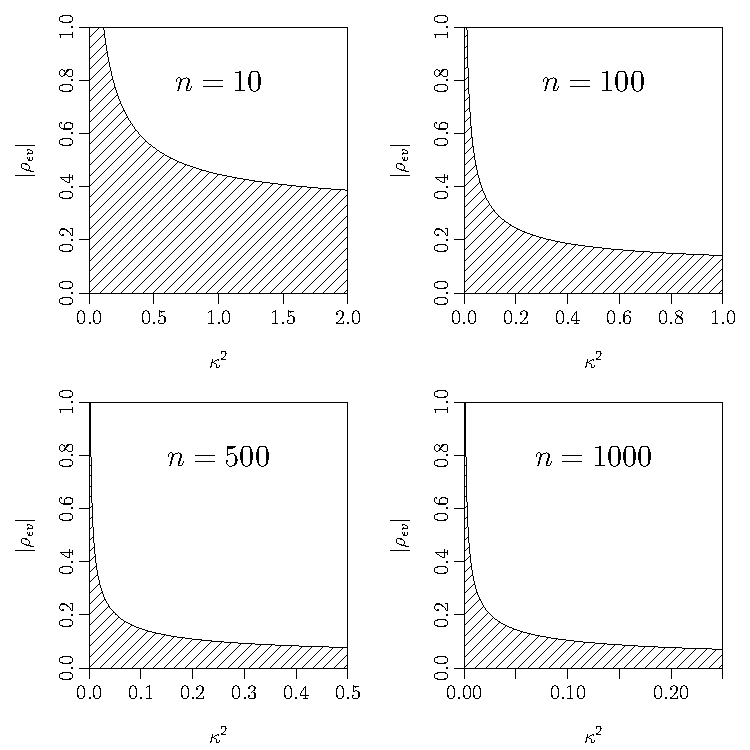
\includegraphics[width=\maxwidth]{figure/OLSboundary} 

\end{knitrout}


% \paragraph{Comparison to Earlier Version:} Notice that these figures look a bit different from the simple example I made earlier for just-identified IV. The difference is the behavior of the boundary near $R^2 = 1$. In the present version the boundary simple asymptotes out of the frame. In the previous version it ``bent inwards'' and intersected the horizontal axis at $R^2 = 1$. (In the earlier version I called this $\rho_{xz}^2$ which is of course equivalent since the first-stage in just-indentified IV is a univariate linear regression.) \emph{So what's going on here?} This boils down to the question of whether the vertical axis should be $\rho_{v\epsilon}$ or $\rho_{x\epsilon}$. In the third line of derivation of the boundary above, we had
  % $$\tau^2 < \sigma_x^2 \sigma_\epsilon^2 \left(\frac{\sigma_x^2}{\gamma^2} - 1\right) $$
% which is the same as
  % $$|\tau|< \sigma_x \sigma_\epsilon \sqrt{\frac{1}{R^2} - 1}$$
% The earlier version used \emph{this} inequality to get the finite-sample rule by working in terms of $\rho_{x\epsilon}$ using $\tau = \sqrt{n} E_n[x_i \epsilon_i] = \sqrt{n} Corr_n(x_i,\epsilon_i) \sigma_x \sigma_\epsilon$. \emph{So what's wrong with that?}. In order for this plot to make sense as a finite-sample interpretation of the FMSC, it needs to be conceptually possible to vary the quantity on the horizontal axis independently of that on the vertical axis. Both the present and earlier versions had the same quantity on the vertical axis: $R^2$. The earlier version had $\rho_{x\epsilon}$ on the vertical axis while the present version has $\rho_{\epsilon v}$. Now, conceptually we're thinking about holding $\sigma_\epsilon$ and $\sigma_v$ fixed. This is what would make the most sense, for example in a simulation study. What we would vary to change the endogeneity of $x$ is the \emph{correlation between} $\epsilon$ and $v$. This much is fine since we can certainly change this correlation without changing the respective variances. The complication comes from $R^2 = (\boldsymbol{\pi}'Q_z \boldsymbol{\pi})/(\boldsymbol{\pi}'Q_z \boldsymbol{\pi} + \sigma_v^2)$. Again, it makes sense to hold $\sigma_v$ fixed, so to change $R^2$ it would make most sense to vary $\mathbf{\pi}$ as, for example, we'd typically think about doing in a simulation. The problem with the earlier version is that changing $\mathbf{\pi}$ \emph{also changes} $\sigma^2_x = \boldsymbol{\pi}'Q_z \boldsymbol{\pi} + \sigma_v^2$ which  \emph{in turn} changes $\rho_{x\epsilon}$. 



\newpage
\begin{assump}[DGP]
\label{assump:local}
  Let $\left\{\left(\mathbf{z}_{ni}', \epsilon_{ni}, v_{ni}\right)'\colon 1\leq i \leq n, n = 1, 2, \hdots\right\}$ be a triangular array of random variables such that $\left(\mathbf{z}_{ni}', \epsilon_{ni}, v_{ni}\right)' \sim \mbox{iid} \;(0, \mathcal{V}_n)$ for fixed $n$ where
		\begin{equation}
		\mathcal{V}_n = \left[ \begin{array}{ccc}
	Q_Z & 0 & 0\\
	0 & \sigma_\epsilon^2 & \tau/\sqrt{n}\\
	0 & \tau/\sqrt{n}& \sigma_v^2
\end{array}	 \right] > 0
		\end{equation}
			\begin{eqnarray}
			y_{ni} &=& \beta x_{ni}  + \epsilon_{ni}\\
	x_{ni} &=& \mathbf{z}_{ni}' \pi + v_{ni}
		\end{eqnarray}
and $\tau,\pi, \beta$ are constants.
\end{assump}


\begin{assump}[Regularity Conditions]
  \label{assump:reg}For some $\eta > 0$,
  \begin{enumerate}[(a)]
		\item $\sup_n E\left[ \lvert\epsilon_iv_i \rvert^{2+\eta}\right]<\infty$ and
		\item $\sup_n E\left[ \lvert \epsilon_{ni} z_{ni\ell} \rvert^{2+\eta} \right]<\infty$ for each component $z_{ni\ell}$ of $\mathbf{z}_{ni}$.
	\end{enumerate}
\end{assump}


For convenience state a Lemma that we'll use for all the limit distributions in the paper. Provides sufficient conditions that specialize the Lindeberg-Feller CLT to the triangular array defined in Assumption \ref{assump:local}. These are basically standard.



\section{Derivations for Choosing Instruments Example}

\begin{eqnarray}
    y_i &=& \mathbf{x}_i' \boldsymbol{\beta} +  \epsilon_i\\
    \mathbf{x}_i &=& \Pi_w \mathbf{w}_i + \Pi_z \mathbf{z}_i + \mathbf{v}_i
\end{eqnarray}

$$E_n[\mathbf{z}_i(y_i - \mathbf{x}_i' \boldsymbol{\beta})] = E_n[\mathbf{z}_i\epsilon_i] = \boldsymbol{\tau}/\sqrt{n}$$

$$E_n[\mathbf{w}_i (y_i - \mathbf{x}_i' \boldsymbol{\beta})]= E_n[\mathbf{w}_i\epsilon_i] = \mathbf{0}$$

$$E_n[\mathbf{x}_i \epsilon_i] = \Pi_z \boldsymbol{\tau}/\sqrt{n} + E_n[\epsilon_i \mathbf{v}_i]$$
Need to think about how to control the endogeneity of $\mathbf{x}$ as I vary other parameters. Perhaps set
  $$E_n[\epsilon_i \mathbf{v}_i] = \boldsymbol{\gamma^2} - \Pi_z \boldsymbol{\tau}/\sqrt{n}$$ so that the endogeneity of $\mathbf{x}$ is held constant at $\boldsymbol{\gamma^2}$? Does this have any effect on the FMSC or does it only matter in the simulation?
  
  Should be able to write this down in terms of a tradeoff 





\end{document}
